\subsection*{Problema 22}

\textbf{Enunciado:} Calcular la integral indefinida
\begin{align*}
\int \dfrac{dx}{\sqrt{-9x^2 + 3x + 4}}
\end{align*}

\textbf{Solución:} Para resolver esta integral, primero completamos el cuadrado dentro de la expresión radical del denominador.

Consideremos la expresión cuadrática:
\begin{align*}
-9x^2 + 3x + 4 &= -9\left(x^2 - \dfrac{1}{3}x\right) + 4
\end{align*}

Completamos el binomio dentro del paréntesis sumando y restando $\left(\dfrac{1}{6}\right)^2 = \dfrac{1}{36}$:
\begin{align*}
-9\left(x^2 - \dfrac{1}{3}x + \dfrac{1}{36} - \dfrac{1}{36}\right) + 4 &= \\
-9\left(x - \dfrac{1}{6}\right)^2 + 9\left(\dfrac{1}{36}\right) + 4 &= \\
-9\left(x - \dfrac{1}{6}\right)^2 + \dfrac{1}{4} + 4 &= \\
-9\left(x - \dfrac{1}{6}\right)^2 + \dfrac{17}{4}
\end{align*}

Sustituyendo esta forma completada en la integral original, obtenemos:
\begin{align*}
\int \dfrac{dx}{\sqrt{\dfrac{17}{4} - 9\left(x - \dfrac{1}{6}\right)^2}}
\end{align*}

Factorizamos $17/4$ dentro de la raíz cuadrada del denominador:
\begin{align*}
\sqrt{\dfrac{17}{4}\left(1 - \dfrac{9}{\frac{17}{4}}\left(x - \dfrac{1}{6}\right)^2\right)} &= \\
\dfrac{\sqrt{17}}{2} \sqrt{1 - \left(\dfrac{3}{\sqrt{17}}\left(x - \dfrac{1}{6}\right)\right)^2}
\end{align*}

Definimos la sustitución:
\begin{align*}
u &= \dfrac{3}{\sqrt{17}}\left(x - \dfrac{1}{6}\right) \\
du &= \dfrac{3}{\sqrt{17}} \, dx \implies dx = \dfrac{\sqrt{17}}{3} \, du
\end{align*}

Sustituyendo en la integral:
\begin{align*}
&\int \dfrac{\frac{\sqrt{17}}{3} \, du}{\frac{\sqrt{17}}{2} \sqrt{1 - u^2}} = \dfrac{2}{3} \int \dfrac{du}{\sqrt{1 - u^2}}
\end{align*}

La integral resultante es directa y corresponde a la función arcoseno:
\begin{align*}
&= \dfrac{2}{3} \arcsin(u) + C
\end{align*}

Reemplazando nuevamente la variable original $x$:
\begin{align*}
&= \dfrac{2}{3} \arcsin\left(\dfrac{3}{\sqrt{17}}\left(x - \dfrac{1}{6}\right)\right) + C \\
&= \dfrac{2}{3} \arcsin\left(\dfrac{6x - 1}{2\sqrt{17}}\right) + C
\end{align*}

\begin{figure}[H]
	\centering
	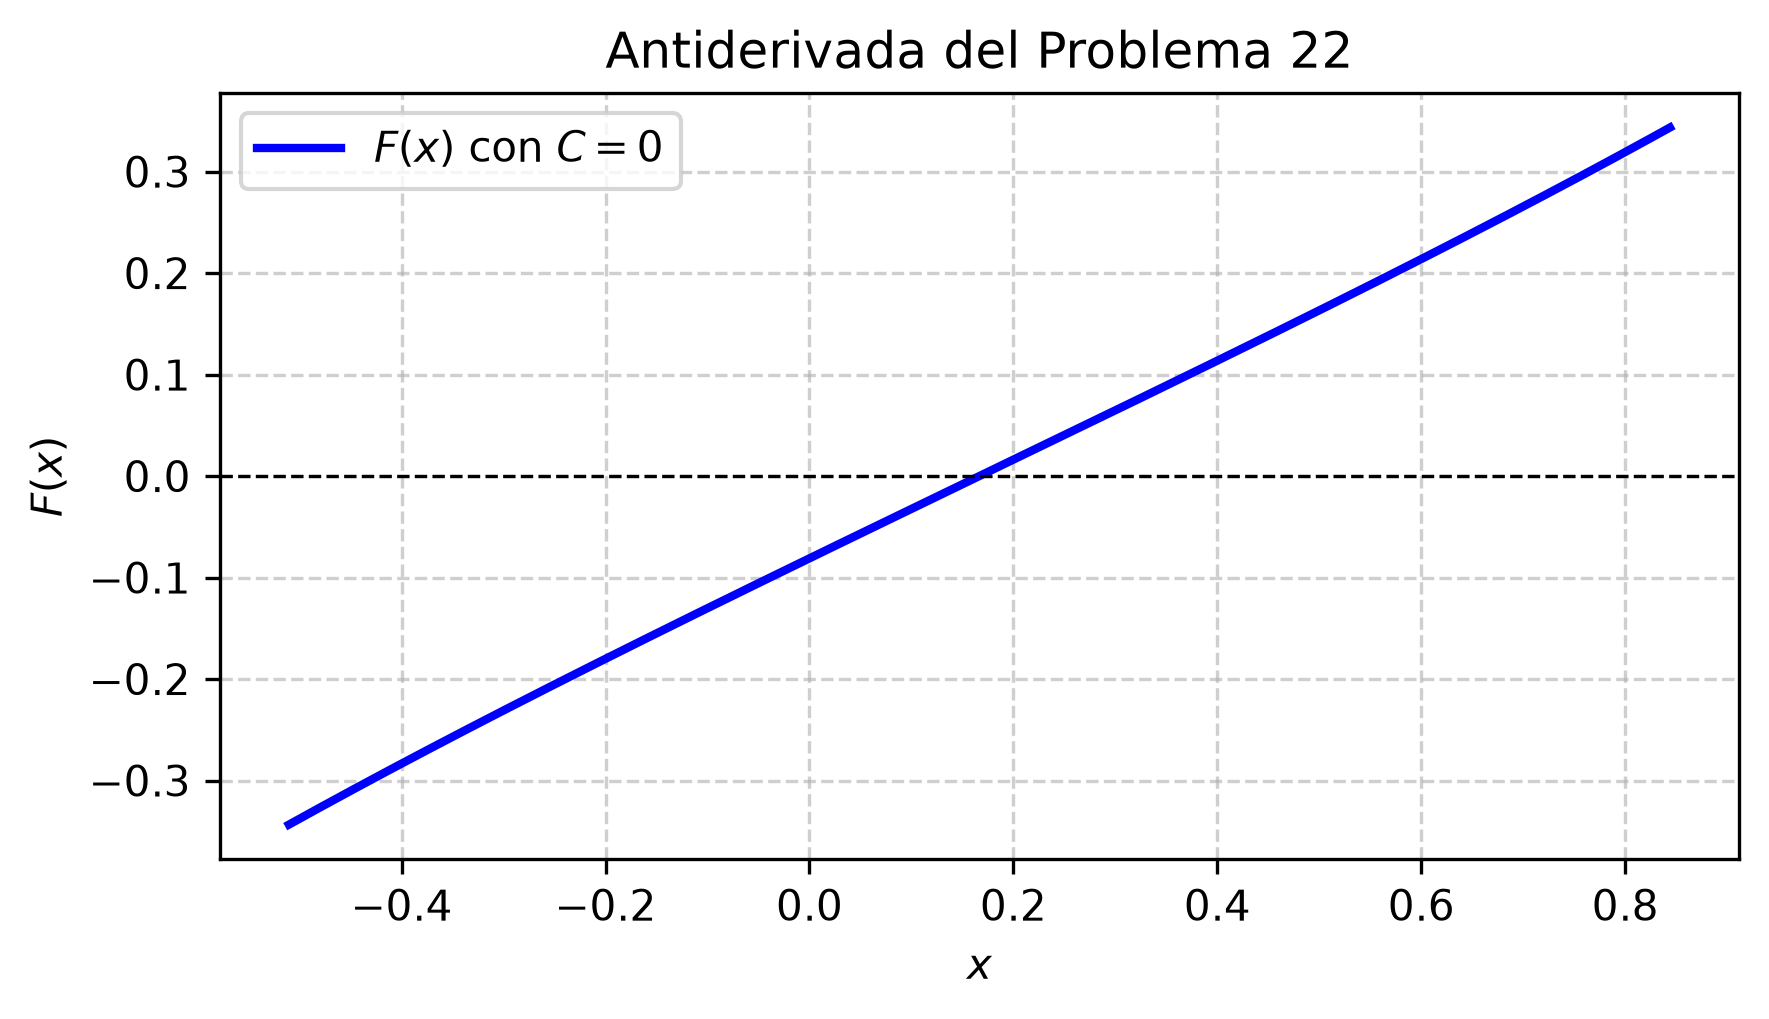
\includegraphics[width=\columnwidth]{semana_05/graficas/SEM05_P22_grafica.png}
	\caption{Representación gráfica de $f(x)$ y su antiderivada $F(x)$ evaluada para la constante de integración $C = 0$ (Problema 22).}
	\label{fig:problema22}
\end{figure}
